% =============================================================================
% CHAPITRE 1 - CINÉMATIQUE
% Partie 11 : Mouvement en deux dimensions
% Version maritime pour l'IMQ
% =============================================================================

% =============================================================================
\section{Mouvement en deux dimensions}
% =============================================================================

Jusqu'\`a pr\'esent, nous avons \'etudi\'e des mouvements en \textbf{une dimension} : des objets se d\'epla\c{c}ant le long d'une ligne droite (un axe $x$ ou $y$). Cependant, la plupart des mouvements r\'eels se produisent en \textbf{deux} ou \textbf{trois dimensions}.

\begin{remarque}[title=Exemples de mouvements en 2D]
\begin{itemize}
    \item Un navire qui navigue sur la mer (surface 2D)
    \item Une balle lanc\'ee qui suit une trajectoire courbe
    \item Un avion en vol (3D, mais on peut souvent simplifier en 2D)
    \item Un homme \`a la mer tomb\'e d'un navire en mouvement
\end{itemize}
\end{remarque}

\subsection{Le principe de d\'ecomposition}

La cl\'e pour analyser un mouvement en 2D est de le \textbf{d\'ecomposer} en deux mouvements ind\'ependants selon les axes $x$ et $y$.

\begin{definition}[title=Ind\'ependance des mouvements]
Dans un mouvement en deux dimensions, les composantes horizontale ($x$) et verticale ($y$) du mouvement sont \textbf{ind\'ependantes} l'une de l'autre.

Cela signifie que :
\begin{itemize}
    \item Le mouvement en $x$ n'affecte pas le mouvement en $y$
    \item Le mouvement en $y$ n'affecte pas le mouvement en $x$
    \item On peut analyser chaque direction s\'epar\'ement
\end{itemize}
\end{definition}

\begin{remarque}[title=Pourquoi peut-on d\'ecomposer? -- D\'evelopper l'intuition]
Cette ind\'ependance semble contre-intuitive! On pourrait penser qu'un objet lanc\'e horizontalement tombe \guillemotleft~moins vite~\guillemotright{} qu'un objet simplement l\^ach\'e. \textbf{C'est faux.}

\textbf{L'exp\'erience des deux balles :}

\begin{center}
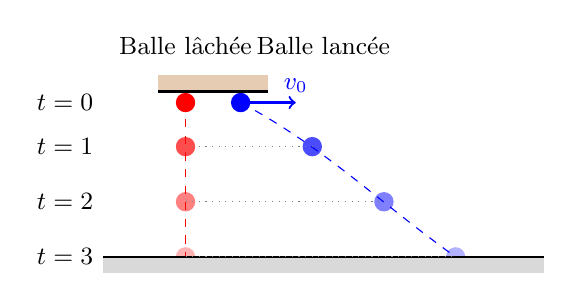
\begin{tikzpicture}[scale=0.7]
% Table
\fill[brown!40] (-1,3) rectangle (1,3.3);
\draw[thick] (-1,3) -- (1,3);
% Balle 1 (lâchée)
\fill[red] (-0.5,2.8) circle (5pt);
\fill[red!70] (-0.5,2) circle (5pt);
\fill[red!50] (-0.5,1) circle (5pt);
\fill[red!30] (-0.5,0) circle (5pt);
\draw[dashed, red] (-0.5,2.8) -- (-0.5,0);
\node[above] at (-0.5,3.5) {\small Balle l\^ach\'ee};
% Balle 2 (lancée)
\fill[blue] (0.5,2.8) circle (5pt);
\fill[blue!70] (1.8,2) circle (5pt);
\fill[blue!50] (3.1,1) circle (5pt);
\fill[blue!30] (4.4,0) circle (5pt);
\draw[dashed, blue] (0.5,2.8) .. controls (2,2) and (3,1) .. (4.4,0);
\draw[thick, blue, ->] (0.5,2.8) -- (1.5,2.8) node[above] {\small $v_0$};
\node[above] at (2,3.5) {\small Balle lanc\'ee};
% Sol
\fill[gray!30] (-2,-0.3) rectangle (6,0);
\draw[thick] (-2,0) -- (6,0);
% Temps
\node[left] at (-2,2.8) {\small $t=0$};
\node[left] at (-2,2) {\small $t=1$};
\node[left] at (-2,1) {\small $t=2$};
\node[left] at (-2,0) {\small $t=3$};
% Lignes horizontales pour montrer la simultanéité
\draw[dotted, gray] (-0.5,2) -- (1.8,2);
\draw[dotted, gray] (-0.5,1) -- (3.1,1);
\draw[dotted, gray] (-0.5,0) -- (4.4,0);
\end{tikzpicture}
\end{center}

Deux balles sont \`a la m\^eme hauteur. Au m\^eme instant, l'une est \textbf{l\^ach\'ee} et l'autre est \textbf{lanc\'ee horizontalement}. R\'esultat : \textbf{elles touchent le sol en m\^eme temps!}

La vitesse horizontale de la balle lanc\'ee n'affecte pas sa chute. Les deux balles subissent exactement la m\^eme acc\'el\'eration verticale ($g$), donc elles tombent \`a la m\^eme vitesse verticale.

\textbf{Analogie maritime :} Imaginez un matelot au sommet d'un m\^at sur un navire avanc ant \`a vitesse constante. S'il l\^ache une cl\'e :
\begin{itemize}
    \item \textbf{Du point de vue du matelot} : la cl\'e tombe droit vers le bas
    \item \textbf{Du point de vue du quai} : la cl\'e suit une trajectoire courbe (parabole)
\end{itemize}
La cl\'e \guillemotleft~conserve~\guillemotright{} la vitesse horizontale du navire pendant toute sa chute, mais cette vitesse horizontale n'affecte en rien la dur\'ee de la chute!

\textbf{Essayez en classe :} Placez deux pi\`eces de monnaie sur le bord d'une table. Frappez-en une horizontalement avec une r\`egle pendant que l'autre tombe. \'Ecoutez : un seul \guillemotleft~clic~\guillemotright{} au sol!
\end{remarque}

\begin{attention}[title=Principe fondamental]
\textbf{Pour r\'esoudre un probl\`eme de mouvement en 2D :}
\begin{enumerate}
    \item D\'ecomposer le mouvement en composantes $x$ et $y$
    \item R\'esoudre \textbf{s\'epar\'ement} le mouvement en $x$ et en $y$
    \item Relier les deux par le \textbf{temps} $\Delta t$ (qui est le m\^eme pour les deux)
    \item Recombiner les r\'esultats si n\'ecessaire
\end{enumerate}
\end{attention}

\subsection{D\'ecomposition d'un vecteur}

Tout vecteur (position, vitesse, acc\'el\'eration) peut \^etre d\'ecompos\'e en composantes :

\begin{center}
\begin{tikzpicture}[scale=1.3]
% Axes
\draw[axe, thick, ->] (0,0) -- (4,0) node[right] {$x$};
\draw[axe, thick, ->] (0,0) -- (0,3) node[above] {$y$};
% Vecteur
\draw[very thick, red, ->] (0,0) -- (3,2) node[above right] {$\vec{v}$};
% Composantes
\draw[thick, blue, ->] (0,0) -- (3,0) node[below] {$v_x$};
\draw[thick, green!60!black, ->] (3,0) -- (3,2) node[right] {$v_y$};
% Angle
\draw[thick] (0.7,0) arc (0:33.7:0.7);
\node at (1,0.3) {$\theta$};
% Rectangle pointillé
\draw[dashed, gray] (0,2) -- (3,2);
\draw[dashed, gray] (0,0) -- (0,2);
\end{tikzpicture}
\end{center}

\begin{equationimportante}
\textbf{D\'ecomposition d'un vecteur}
\begin{align}
v_x &= v \cos\theta \\
v_y &= v \sin\theta
\end{align}
o\`u $\theta$ est l'angle par rapport \`a l'horizontale.

\textbf{Recomposition (module et direction)}
\begin{align}
v &= \sqrt{v_x^2 + v_y^2} \\
\theta &= \arctan\left(\frac{v_y}{v_x}\right)
\end{align}
\end{equationimportante}

\subsection{Exemple : navigation d'un navire}

\begin{exemple}{Cap et vitesse d'un navire}{}
Un navire navigue \`a $\SI{15}{n\oe{}uds}$ avec un cap de $30°$ par rapport \`a l'est (c'est-\`a-dire $30°$ nord de l'est).

Quelles sont les composantes est-ouest et nord-sud de sa vitesse?

\begin{center}
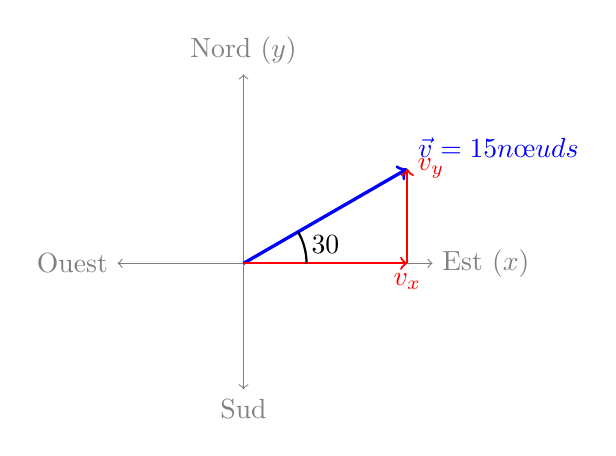
\begin{tikzpicture}[scale=0.8]
% Rose des vents simplifiée
\draw[gray, ->] (0,0) -- (3,0) node[right] {Est ($x$)};
\draw[gray, ->] (0,0) -- (0,3) node[above] {Nord ($y$)};
\draw[gray, ->] (0,0) -- (-2,0) node[left] {Ouest};
\draw[gray, ->] (0,0) -- (0,-2) node[below] {Sud};
% Vecteur vitesse
\draw[very thick, blue, ->] (0,0) -- (2.6,1.5) node[above right] {$\vec{v} = \SI{15}{n\oe{}uds}$};
% Composantes
\draw[thick, red, ->] (0,0) -- (2.6,0) node[below] {$v_x$};
\draw[thick, red, ->] (2.6,0) -- (2.6,1.5) node[right] {$v_y$};
% Angle
\draw[thick] (1,0) arc (0:30:1);
\node at (1.3,0.3) {$30°$};
% Navire
\node at (1.3,0.75) {\small $\blacktriangle$};
\end{tikzpicture}
\end{center}

\textbf{Composante est-ouest :}
\[ v_x = v \cos\theta = 15 \cos 30° = 15 \times 0,866 = \SI{13,0}{n\oe{}uds} \]

\textbf{Composante nord-sud :}
\[ v_y = v \sin\theta = 15 \sin 30° = 15 \times 0,5 = \SI{7,5}{n\oe{}uds} \]

Le navire se d\'eplace donc \`a $\SI{13,0}{n\oe{}uds}$ vers l'est et $\SI{7,5}{n\oe{}uds}$ vers le nord.
\end{exemple}

\subsection{Application au projectile}

Le mouvement d'un \textbf{projectile} (objet lanc\'e dans l'air) est l'exemple classique de mouvement en 2D. On le d\'ecompose en :

\begin{center}
\renewcommand{\arraystretch}{1.5}
\begin{tabular}{|c|c|}
\hline
\rowcolor{bleuclair}
\textbf{Direction horizontale ($x$)} & \textbf{Direction verticale ($y$)} \\
\hline
Aucune force horizontale & Gravit\'e (vers le bas) \\
\hline
$a_x = 0$ & $a_y = -g$ \\
\hline
\textbf{MRU} (vitesse constante) & \textbf{Chute libre} (MRUA) \\
\hline
\end{tabular}
\end{center}

\begin{remarque}[title=Ce qui relie les deux directions]
Les mouvements en $x$ et en $y$ sont ind\'ependants, mais ils partagent le m\^eme \textbf{temps} $\Delta t$.

C'est cette variable commune qui permet de relier les deux directions et de d\'eterminer, par exemple, o\`u un projectile atterrit.
\end{remarque}

Dans la section suivante, nous appliquerons ces principes \`a l'\'etude compl\`ete du mouvement d'un projectile.
